\documentclass[nofootinbib,amssymb,amsmath]{revtex4}
\usepackage{mathtools}
\usepackage{amsthm}
\usepackage{algorithm}
\usepackage{algpseudocode}
\usepackage{lmodern}
\usepackage{graphicx}
\usepackage{color}

\newcommand{\RCS}{\texttt{ReCapSeg}}
\newcommand{\ACS}{\texttt{AllelicCapSeg}}

%Put an averaged random variable between brackets
\newcommand{\ave}[1]{\left\langle #1 \right\rangle}

\newtheorem{lemma}{Lemma}
\newtheorem{corollary}{Corollary}

\def\SL#1{{\color [rgb]{0,0,0.8} [SL: #1]}}
\def\DB#1{{\color [rgb]{0,0.8,0} [DB: #1]}}

\begin{document}

\title{Notes on $\ACS$}
\author{Samuel K. Lee}
\affiliation{Broad Institute, 75 Ames Street, Cambridge, MA 02142}
\email{slee@broadinstitute.org}
\date{\today}

\begin{abstract}
Some notes on the methods used in the current \texttt{python} implementation and proposed methods for the \texttt{hellbender}
port.
\end{abstract}

\maketitle



\section{Introduction}\label{introduction}

\SL{A brief intro here would be nice.}

\section{$\RCS$ Overview} \label{recapseg-overview}

We first summarize the portions of the $\RCS$ workflow that generate the input for $\ACS$.  The below is copied/paraphrased from the documentation at \url{http://gatkforums.broadinstitute.org/discussion/5640/recapseg-overview}.

$\RCS$ is a copy-number--variant detector that runs on user-defined target regions, which can correspond to exomes, gene panels, or arbitrary windows. $\RCS$ uses a Panel of Normal (PoN) samples to model noise and normalize the coverage calls of the target sample. These methods were designed for copy-number calling (amplification and deletion) of somatic events with a resolution of two or more targets. $\RCS$ does not need a matched normal, but operates on a panel of normal samples representing similar library preparation to agnostically remove noise. $\RCS$ is the production version of the \texttt{CapSeg} algorithm.

Given an DNA-Seq alignment BAM file and a BED file of target genomic intervals, the $\RCS$ algorithms estimate copy ratio by performing the following steps:

\begin{enumerate}
\item
Generate proportional coverage: First, the per sample normalized coverage is calculated by normalizing the read coverage spanning a
target segment with the total number of aligned reads (for every read group: number of reads over segment/total number of aligned reads).  The proportional coverage is then calculated by normalizing every segment with the median normalized coverage across the PoN for the given segment.
\item
Tangent normalization: This normalization procedure projects the sample proportional coverage to a hyperplane defined by the PoN. This normalization procedure results in a copy-ratio estimate with reduced noise.
\item
Segment: The target regions are then merged into continuous segments that represent the same copy-number event. The segmentation is performed by a circular-binary-segmentation (CBS) algorithm described by Olshen et al. 2004 that was originally developed to segment noisy array copy-number data.\footnote{Specifically, the CBS implementation provided by the \texttt{R} package \texttt{DNACopy} is used. Note that even though the \texttt{DNACopy} parameter \texttt{data.type} is set to \texttt{logratio}, the tangent-normalized \emph{linear} copy ratios are used instead.  \SL{Check this?  If true, it is unclear to me how this affects the resulting segmentation, if at all.}} Currently, $\RCS$ considers only segments that include two or more targets (a target usually represents a single exon).
\end{enumerate}

To summarize, given coverage data for a set of targets, $\RCS$ produces 1) $\log_2$ copy-ratio estimates for each target, and 2) corresponding segments, which are specified by a set of genomic intervals.  The segment files produced by $\RCS$ also contain segment ``means,'' which are given by the mean linear copy ratio of all targets contained within each segment.

\section{Current Hellbender $\ACS$ Workflow} \label{current-alleliccapseg-workflow}

\subsection{Segmented model} \label{segmented-model}
We want a generative model for allelic fractions that infers its parameters from the data.  We observe alt and ref read counts for each het site and wish to infer the minor allelic fraction of every segment.  Let's consider what other hidden variables belong in the model.  Read counts obey an overdispersed binomial distribution in which the probability of an alt read is a site-dependent random variable.  Letting $\theta_j$ be the probability that a mapped read at het $j$ is an alt we have
%
\begin{equation}
P(a_j, r_j | \theta_j) =  \binom{a_j + r_j}{a_j} \theta_j^{a_j} (1-\theta_j)^{r_j} = \binom{n_j}{a_j} \theta_j^{a_j} (1-\theta_j)^{r_j},
\end{equation}
where $a_j$ and $r_j$ are alt and ref read counts and $n_j = a_j + r_j$ is the total read count at site $j$.  Now we consider $\theta_j$.  Suppose site $j$ belongs to a segment with minor allelic fraction $f$ and is alt minor, such that $P({\rm alt}) = f$ and $P({\rm ref}) = 1 - f$ are the probabilities that a random DNA fragment will contain the alt and ref alleles.  Let $x^{\rm alt (ref)}_j = P({\rm mapped} | {\rm alt (ref)})$ be the probabilities that an alt (ref) DNA fragment at site $j$ eventually gets sequenced and mapped.  Then $\theta_j$ is the conditional probability that a mapped read comes from an alt fragment:
%
\begin{align}
\theta_j  &= P( {\rm alt} | {\rm mapped} ) = \frac { P( {\rm alt} ) P( {\rm mapped} | {\rm alt} ) } { P( {\rm alt} ) P( {\rm mapped} | {\rm alt} ) + P( {\rm ref} ) P( {\rm mapped} | {\rm ref} ) } \\
 &= \frac{f x^{\rm alt}_j }{fx^{\rm alt} + (1-f) x^{\rm ref}_j } = \frac{f}{f + (1-f) \lambda_j},
\end{align}
%
where $\lambda_j = x^{\rm ref}_j / x^{\rm alt}_j$ is the ``bias ratio'' of ref to alt sequenceability and mappability at site $j$.  A similar result for ref minor sites follows from substituting $f \leftrightarrow 1 - f$.  In addition to the bias ratio $\lambda_j$ we need an indicator variables $z_j$ with three states, alt minor, ref minor, and an outlier state that gives robustness to anomalous events.  For this outlier state we average the binomial likelihood over all $\theta$ to get:
%
\begin{align}
P(a_j, r_j | {\rm outlier}) = \binom{n_j}{a_j} \int_0^1 \theta_j^{a_j} (1-\theta_j)^{r_j} \, d \theta_j 
= \binom{n_j}{a_j} \frac{a_j! r_j!}{(n_j + 1)!}
\end{align}
%
For notational convenience we give $z_j$ a one-of-$K$ encoding $z_j = (z_{ja}, z_{jr}, z_{jo})$ in which one component equals $1$ and the rest $0$.

The contribution of site $j$ to the likelihood is
%
\begin{equation}
P(a_j, r_j | f_j, \lambda_j, z_j) =  \binom{n_j}{a_j}  
\left[ \frac{f_j^{a_j} (1 - f_j)^{r_j} \lambda_j^{r_j}}{ \left( f_j + (1-f_j) \lambda_j \right)^{n_j}} \right]^{z_{ja}}   
\left[ \frac{(1-f_j)^{a_j} f_j^{r_j} \lambda_j^{r_j}}{ \left( 1 - f_j + f_j \lambda_j \right)^{n_j}} \right]^{z_{jr}}   
\left[ \frac{a_j! r_j!}{(n_j + 1)!} \right]^{z_{jo}}
\label{likelihood}
\end{equation}
%
where $f_s$ is the minor allele fraction of the segment containing site $j$.  We will consider $f$ to be drawn from a uniform distribution on $[0, 1/2]$ -- that is, we give it a flat prior -- but in the future we can obtain some sort of clustering behavior, representing the fact that events in the same subclone that exhibit the same integer copy numbers will have the same minor allelic fractions, by drawing $f_s$ from a Dirichlet process.

We assume that the bias ratios come from a common Gamma distribution with parameters $\alpha, \beta$:
%
\begin{equation}
P(\lambda_j | \alpha, \beta) = \frac{\beta^\alpha}{\Gamma(\alpha)} \lambda_j^{\alpha-1} e^{-\beta \lambda_j}
\end{equation}
%
Note that bias ratios tend to be near $1.0$ and so the choice of distribution is not too important as long as it has adjustable mean and standard deviation.  We choose the Gamma distribution because it is the simplest such distribution on $\mathbb{R}^+$.  We will give the parameters $\alpha$ and $\beta$ a flat prior $P(\alpha, \beta) \propto 1$.

Finally, the indicator $z_j$ is a multinomial random variable distributed according to parameter vector ${\bf \pi}$:
%
\begin{equation}
P(z_{ja(r,o)} = 1 | {\bf \pi}) = \pi_{a(r,o)}
\end{equation}
We set the alt and ref minor probabilities equal so that the only free parameter is $\pi = \pi_o$, with $\pi_{a(r)} = (1 - \pi)/2$.
%
The Bayesian network corresponding to this model is shown in Figure \ref{graphical_model}.
\begin{figure}
$
\begin{array}{c}
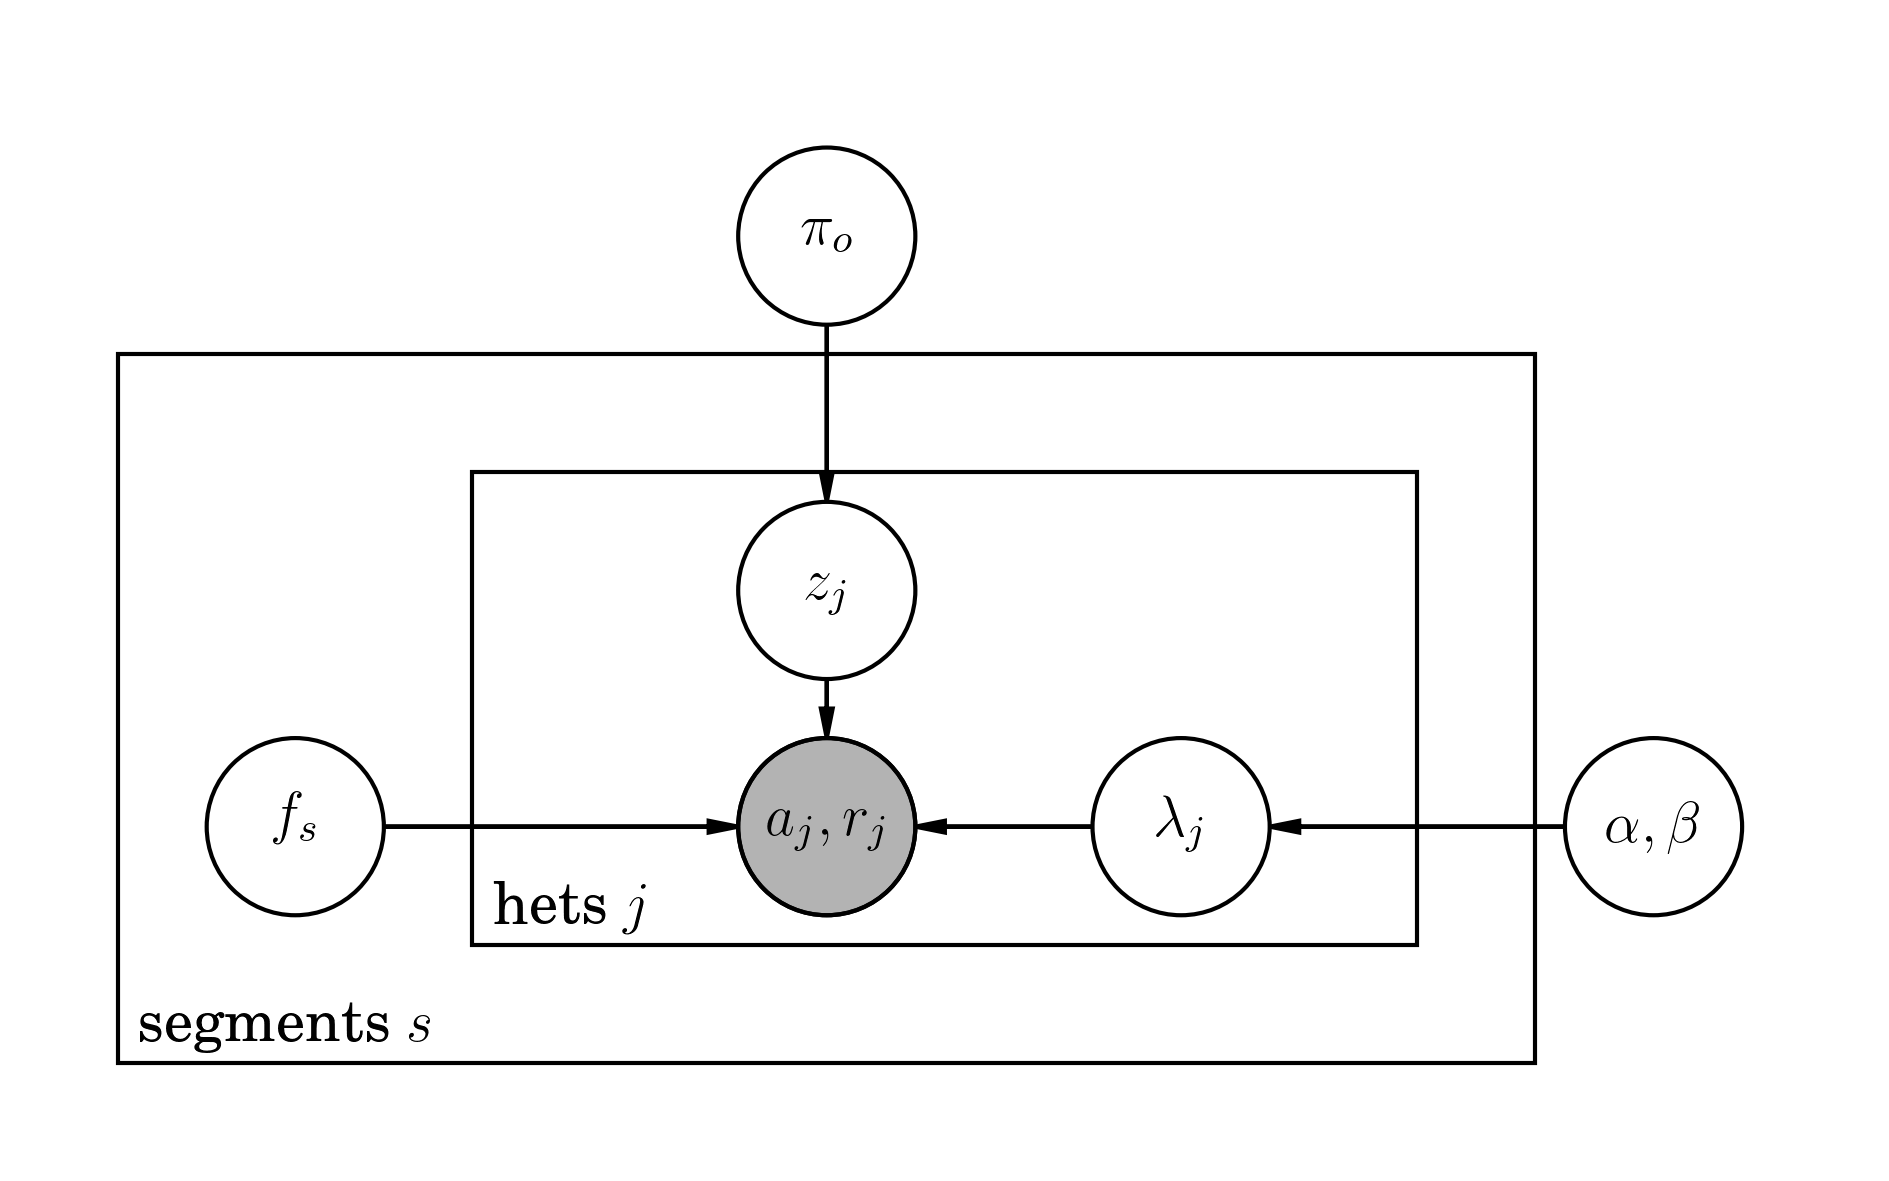
\includegraphics[width=0.8\linewidth]{ACS_model.png} 
\end{array}
$
\label{graphical_model}
\caption{Graphical model for \ACS} 
\end{figure}

As with the other parameters, we put a flat prior on ${\rm \pi}$.  Putting all the pieces together the likelihood is
\begin{equation}
\mathbb{L} =\prod_j \frac{\beta^\alpha}{\Gamma(\alpha)} \lambda_j^{\alpha - 1} e^{-\beta \lambda_j}
\left[ \frac{(1-\pi) f_j^{a_j} (1 - f_j)^{r_j} \lambda_j^{r_j}}{ \left( f_j + (1-f_j) \lambda_j \right)^{n_j}} \right]^{z_{ja}}   
\left[ \frac{(1-\pi) (1-f_j)^{a_j} f_j^{r_j} \lambda_j^{r_j}}{ \left( 1 - f_j + f_j \lambda_j \right)^{n_j}} \right]^{z_{jr}}   
\left[ \frac{2 \pi a_j! r_j!}{(n_j + 1)!} \right]^{z_{jo}}.
\label{likelihood}
\end{equation}
%
The dependence on $\lambda$ for alt minor sites is
%
\begin{equation}
g(\lambda_j, \alpha, \beta, f_j, a_j, r_j) = \frac{\beta^\alpha}{\Gamma(\alpha)}  \frac{ f_j^{a_j} (1 - f_j)^{r_j}  \lambda_j^{\alpha + r_j - 1} e^{-\beta \lambda_j}}{ \left( f_j + (1-f_j) \lambda_j \right)^{n_j}}.
\end{equation}
For ref minor sites the dependence is the same but with $f \leftrightarrow 1 - f$.  We show in show in Appendix \ref{marginalizing} that this function can be integrated analytically, and thus we can marginalize $\lambda$ out of the model to obtain the likelihood
%
\begin{equation}
\prod_j 
\left[ \frac{1-\pi}{2} \phi(\alpha, \beta, f_j, a_j, r_j)  \right]^{z_{ja}}   
\left[ \frac{1-\pi}{2} \phi(\alpha, \beta, 1 - f_j, a_j, r_j)  \right]^{z_{jr}}   
\left[ \frac{ \pi a_j! r_j!}{(n_j + 1)!}  \right]^{z_{jo}},
\label{marginalized}
\end{equation}
%
where $\phi(\alpha, \beta, f_j, a_j, r_j) = \int_0^\infty g(\lambda, \alpha, \beta, f, a, r) \, d \lambda_j$.  Pseudocode for computing $\phi$ is presented in Appendix \ref{marginalizing}.  Furthermore, marginalizing out $z$ is trivial -- simply sum each term over its three possible states.  We then have a collapsed likelihood
%
\begin{equation}
p(f,\alpha, \beta, \pi) \propto \prod_j 
\left[    \frac{1-\pi}{2} \phi(\alpha, \beta, f_j, a_j, r_j)  +
\frac{1-\pi}{2} \phi(\alpha, \beta, 1 - f_j, a_j, r_j)  +
 \frac{ \pi a_j! r_j!}{(n_j + 1)!}    \right]
 \label{collapsed}
\end{equation}
%
Integrating out the latent variables removes the strongest correlations from the model -- intuitively, $f$ should not be too sensitive to $\alpha$ and $\beta$, for example -- and significantly improves mixing.  The exception is $\alpha$ and $\beta$, since adjusting one with the other fixed changes the mean of the prior on $\lambda$.  Thus we reparameterize in terms of $\mu$ and $\beta$, where $\alpha = \mu \beta$ ($\mu$ is the mean of ${\rm Gamma}(\alpha, \beta)$.  Due to the weak correlations our MCMC method does not need to be very sophisticated.  We choose to sample each variable with one-dimensional adaptive Metropolis, tuning the proposal step size to achieve some reasonable acceptance rate like $0.4$ or so.  Thus we have completely specified an MCMC scheme for this model, given by Algorithm \ref{ACS_MCMC}:

\begin{algorithm}
\begin{algorithmic}[1]
\ForAll{segments $s$}
	\State Initialize $f_s = \sum_{j \in s} {\rm min}(a_j, r_j) / \sum_{j \in s} n_j$
\EndFor
\State Initialize $\mu = 1$
\State Initialize $\beta = 10$
\State Initialize $\pi = 0.01$
\Repeat
	\State Sample each $f_s$ with adaptive Metropolis
	\State Sample $\pi$ with adaptive Metropolis
	\State Sample $\mu$ with adaptive Metropolis
	\State Sample $\beta$ with adaptive Metropolis
\Until{convergence}
\end{algorithmic}
\caption{MCMC algorithm for \ACS}
\label{ACS_MCMC}
\end{algorithm}

\subsection{Target/SNP segment union} \label{targetsnp-segment-union}

\SL{DB can fill this in.}

\subsection{Small-segment merging} \label{small-segment-merging}

\SL{SL to update this to the new method.}

Using CBS to segment the targets in $\RCS$ results in segments that are \SL{always?} larger than $\sim$2--3 targets.  However, after taking the union of target and SNP segments, small segments with less than $\sim$2--3 targets may be introduced.  To be consistent with CBS and $\RCS$, $\ACS$ treats these small segments as spurious, and removes them by merging them with adjacent segments.

A segment is considered to be small if the number of targets it contains is strictly less than a threshold number of targets $n_t$; we take $n_t = 3$.  The small-segment merging algorithm checks each $i$th segment in turn, starting with the first, leftmost segment.  If the segment is small, it is repeatedly merged with the adjacent segment that is closer in the $L_1$ distance $|\tau_i - \tau_{i \pm 1}| + |f_i - f_{i \pm 1}|$ in copy-ratio--allele-fraction space until it is no longer small.\footnote{To be explicit, segments are reindexed after each merge, so that the new segment formed by merging segment $i$ and segment $i \pm 1$ retains the index $i$.}  Exceptions occur for adjacent segments on different chromosomes, which are never merged; in practice, this is enforced by setting the $L_1$ distance between segments on different chromosomes to be infinite.  After all segments have been checked and merged, any remaining small segments (which will be present if any chromosome contains less than $n_t$ targets) are dropped.

\subsection{Parameter optimization}\label{parameter-optimization}

\subsection{Similar-segment merging} \label{similar-segment-merging}

\subsection{Final parameter optimization} \label{final-parameter-optimization}

\section{Proposed Methods for $\texttt{hellbender}$} \label{proposed-methods-for-texttthellbender}

\subsection{Bayesian het pulldown} \label{bayesian-het-pulldown}

We are given a large data set of ref and alt read counts over many potential SNP sites and we wish to infer which sites are hets and with what probabilities.  This problem is naturally represented as a mixture model in which the hidden labels are genotypes -- hom ref, het, and hom alt.  Since the observed data are ref and alt counts is seems natural to use a binomial mixture model in which the binomial parameters are the probability of an alt read.  Then the binomial parameters are the error rate for hom ref genotypes, $1/2$ times the allelic bias for het genotypes, and $1$ minus the error rate for hom alt genotypes.  However, actual data are overdispersed because the error rate and allelic bias are random variables, not single parameters.  For example, sequencing error rates and allelic bias (for concreteness, consider mapping bias) depend on context.  Thus a beta-binomial mixture model is more appropriate.  A maximum-likelihood (MLE) approach will yield posterior probabilities on the genotypes at each locus, in particular the het probability.  It also gives the parameters of a beta distribution of allelic bias, which is useful downstream in ACS.

For generality and at no cost in complexity, consider a Dirichlet-multinomial mixture (DMM) with $K$ mixture components and $M$ classes of observed data.  For our purposes there are $K = 3$ genotypes and $M = 2$ types of read, ref and alt.  The beta-binomial distribution is the $M = 2$ case of the Dirichlet-multinomial.  The observed data are counts $n_{jm}$, the number of times class m was seen in observation $j$.  For us, each potential SNP site is a datum $j$.  Let $N_j = \sum_m n_{jm}$ denote the total read count at site $j$.  For our purposes, $\{ N_j \}$ are constants -- we are not trying to model depth of coverage here, just the proportions of the coverage allotted to ref and alt reads.

We represent hidden labels via the 1-of-$K$ encoding ${\bf z}_j = (0, 0, \ldots 1, 0, 0 \ldots)$, so $z_{jk} = 1$ when datum j comes from component $k$.  The hidden labels are multinomially distributed as $P({\bf z}_j) = {\rm Mult}({\bf z}_j | {\bf \pi})$, where $\pi_k$ is the probability of component $k$ and $\sum_k \pi_k = 1$.  Finally, the observed counts for mixture component $k$ are drawn from a Dirichlet-multinomial distribution with parameter ${\bf \alpha}_k$:

\begin{equation}
P({\bf n}_j \mid z_{jk} = 1, {\bf \alpha}_k ) = \frac{ \Gamma (A_k) }{ \Gamma (A_k + N_j) } \prod_m \frac{ \Gamma (\alpha_{km} + n_{jm}) }{ \Gamma (\alpha_{km}) },
\end{equation}
where $A_k = \sum_m \alpha_{km}$.

The EM algorithm for MLE estimates of $\{ \pi_k \}$ and $\{ \alpha_{km} \}$ requires the complete-data likelihood (CDL), that is, the joint likelihood of the observed data and hidden labels given the parameters.  In contrast, a direct approach maximizes the likelihood marginalized over the hidden variables.  The CDL of of the DMM is
\begin{align}
P({\bf z}, {\bf n} \mid {\bf \pi}, {\bf \alpha}) = & P({\bf z} \mid {\bf \pi}) P({\bf n} \mid {\bf z}, {\bf \alpha}) \\
= & \prod_{jk}  \left[ \pi_k \frac{ \Gamma (A_k) }{ \Gamma (A_k + N_j) } \prod_m \frac{ \Gamma (\alpha_{km} + n_{jm}) }{ \Gamma (\alpha_{km}) } \right]^{z_{jk}} \label{CDL}
\end{align}

In the E step of the EM algorithm, we obtain the posterior distribution on $P({\bf z} \mid {\bf n}, {\bf \pi}, {\bf \alpha})$ from Eq. (\ref{CDL}).  By inspection the posterior is a product of independent multinomials
\begin{equation}
\label{DMM_E_step}
\bar{z}_{jk} \equiv P(z_{jk} = 1 \mid {\bf n}, {\bf \pi}, {\bf \alpha})  \propto \pi_k \frac{ \Gamma (A_k) }{ \Gamma (A_k + N_j) } \prod_m \frac{ \Gamma (\alpha_{km} + n_{jm}) }{ \Gamma (\alpha_{km}) },
\end{equation}
with a normalization constant determined by the condition $\sum_k \bar{z}_{jk} = 1$.

In the M step of the EM algorithm we take the expectation of the log-CDL with respect to the posterior on ${\bf z}$ and maximize with respect to ${\bf \pi}$ and ${\bf \alpha}$.  That is, we maximize
\begin{equation}
\sum_{jk}  \bar{z}_{jk} \left\{ \log \pi_k + \log \frac{\Gamma (A_k)}{ \Gamma (A_k + N_j)}  + \sum_m \log \frac{ \Gamma (\alpha_{km} + n_{jm})}{\Gamma (\alpha_{km})}  \right\}.
\end{equation}

Maximizing with respect to $\pi_k$ with a Lagrange multiplier for the constraint $\sum_k \pi_k = 1$
\begin{equation}
\label{DMM_M_step_pi}
\pi_k = \frac{ \sum_j \bar{z}_{jk} }{\sum_{j \ell} \bar{z}_{j \ell}}
\end{equation}

To maximize with respect to ${\bf \alpha}$ we use the fact that if we are trying to maximize $f({\bf x})$ and have a current guess of ${{\bf x}_0}$, then an improved guess may be obtained by maximizing $g({\bf x})$, where $g({\bf x}_0) = f({\bf x}_0)$ and $g({\bf x}) \le f({\bf x})$ for all ${\bf x}$.  Furthermore, repeating this gives an iterative optimization that converges to a local maximum.  Using bounds (\ref{bound1}) and (\ref{bound2}) and dropping additive constants, we find that the iterative step is to maximize the lower bound
\begin{equation}
\sum_{jk}  \bar{z}_{jk} \left\{ - \left( \psi(\hat{A}_k + N_j) - \psi(\hat{A}_k) \right) A_k + \sum_m \hat{\alpha}_{km}  \left( \psi(\hat{\alpha}_{km}  + n_{jm}) - \psi(\hat{\alpha}_{km}) \right)  \log(\alpha_{km} )   \right\}.
\end{equation}
with respect to $\alpha_{km}$ treating the ``old'' guesses $\hat{\alpha}_{km}$ as constants.  This maximization is a straightforward matter of setting the derivative to zero and gives the fixed-point iteration
\begin{equation}
\label{DMMiteration}
\alpha_{km} = \hat{\alpha}_{km} \frac{\sum_j \bar{z}_{jk}  \left( \psi(\hat{\alpha}_{km}  + n_{jm}) - \psi(\hat{\alpha}_{km}) \right)} {\sum_j \bar{z}_{jk} \left( \psi(\hat{A}_k + N_j) - \psi(\hat{A}_k) \right)}
\end{equation}

As is often the case with mixture models, we risk converging to a bad local maximum if parameters are initialized poorly.  Following the approach used by Thomas Minka in his FastFit software, we obtain a good initial guess by fitting a Dirichlet mixture model (as opposed to a Dirichlet-multinomial model) on effective multinomial pseudodata.  That is, instead of working with \textit{counts} $n_{jm}$, work with \textit{proportions} $p_{jm} = n_{jm} / N_j$.  Since $\sum_m p_{jm} = 1$, ${\bf p}_j$ can be interpreted as a multinomial distribution drawn from a Dirichlet mixture.  This preprocessing step maps the original count data onto the $(M-1)$-dimensional simplex, and we can then assign the pseudo-multinomials $\{ {\bf p}_j \}$ to $K$ clusters via the $K$-means algorithm.  Define the indicator variable $\chi_{jk} = 1$ if pseudo-multinomial ${\bf p}_j$ is assigned to cluster $k$ and let $\chi_{jk} = 0$ otherwise.

We initialize $\pi_k$ as the empirical proportion of mixture component $k$ in the clustering step.  That is
\begin{equation}
\label{DMM_initialize_pi}
\pi_k = \frac{\sum_j \chi_{jk}}{N} = \frac{N_k}{N}
\end{equation}
where $N_k$ is the number of pseudo-multinomials assigned to cluster $k$.

Then for each component $k$ we initialize the Dirichlet parameter vector ${\bf \alpha_k}$ via moment matching.  Parameterize ${\bf \alpha_k}$ as ${\bf \alpha}_k = s_k {\bf \theta}_k$, where $\sum_m \theta_{km} = 1$ is the mean of the Dirichlet distribution and $s$ is its concentration.  Since multinomials $S_k = \{ {\bf p}_j \, : \, \chi_{jk} = 1 \}$ are presumed drawn from Dirichlet distribution with parameter ${\bf \alpha}_k$, we set the theoretical mean ${\bf \theta}_k$ to the empirical mean of $S_k$:
\begin{equation}
\theta_{km} = \left\langle   {\bf p}_j \in S_k \right\rangle = \frac{1}{N_k} \sum_j \chi_{jk} p_{jm}
\label{1st_moment_matching}
\end{equation}

Moment matching of the $m$-th diagonal component of the covariance gives
\begin{align}
\frac{ \alpha_{km} \left( \sum_\ell \alpha_{k \ell} - \alpha_{km} \right) }{\left( \sum_\ell \alpha_{k \ell}\right)^2 \left( \sum_\ell \alpha_{k \ell} + 1 \right) }=& {\rm cov}(S_k)_{mm} =  \left\langle   p_{jm}^2 \in S_k \right\rangle - \left\langle   p_{jm} \in S_k \right\rangle^2 \\
%
\frac{ \theta_{km} (1 - \theta_{km})} {s_k + 1} =& \frac{1}{N_k} \sum_j \chi_{jk} p^2_{jm} \\
s_k = & \frac{  \theta_{km} - \frac{1}{N_k} \sum_j \chi_{jk} p^2_{jm}}{\frac{1}{N_k} \sum_j \chi_{jk} p^2_{jm} - \theta_{km}^2 }
\label{2nd_moment_matching}
\end{align}

Since these $M$ estimates $s_k$ do not need to agree, we simply take their average.


The EM algorithm for DMM inference is summarized in Algorithm \ref{DMM}.

\begin{algorithm}
\begin{algorithmic}[1]
\State Form pseudo-multinomial data $p_{jm} = n_{jm} / N_j$
\State Find $K$ clusters of this pseudodata via the $K$-means algorithm.
\State Initialize ${\bf \pi}$ via Eq. \ref{DMM_initialize_pi}
\State Initialize $\{ \alpha_{km} \}$ via Eqs. \ref{1st_moment_matching} and \ref{2nd_moment_matching}
\Repeat
	\State Update $\bar{z}_{jk}$ via Eq. \ref{DMM_E_step}
	\State Update ${ \bf \pi}$ via Eq. \ref{DMM_M_step_pi}
		\Repeat
		\State update $ \{ \alpha_{km} \}$ via Eq. \ref{DMMiteration}
	\Until{convergence}
\Until{convergence}
\end{algorithmic}
\caption{EM algorithm for Dirichlet-multinomial mixture model}
\label{DMM}
\end{algorithm}

Returning to our original task, we obtain three mixture components with Dirichlet parameters $(\alpha_{k1}, \alpha_{k2})$.  The mean proportion of alt reads (WLOG we choose $m = 1$ to be alt and $m=2$ to be ref) are $\alpha_{k1}/(\alpha_{k1} + \alpha_{k2})$, so we can assign mixture labels $k = 1, 2, 3$ to genotypes by comparing these proportions to $0$ (hom ref), $1/2$ (het) and $1$ (hom alt). The posterior probability $\bar{z}_{jk}$ is the probability that site $j$ has genotype $k$, which is exactly what we need for a probabilistic het pulldown.

\subsection{Model-comparison test for segment merging} \label{likelihood-based-segment-merging}

\SL{I'll fill this in once it's worked out.}

%%%APPENDICES
\appendix

\section{Marginalizing out latent variables of the \ACS model} \label{marginalizing}
We wish to evaluate
%
\begin{equation}
\phi(\alpha, \beta, f, a, r) = \int_0^\infty g(\lambda, \alpha, \beta, f, a, r) \, d \lambda 
\end{equation}
%
where
%
\begin{equation}
g(\lambda, \alpha, \beta, f, a, r) =  \frac{\beta^\alpha}{\Gamma(\alpha)}  \frac{ f_j^{a} (1 - f)^{r}  \lambda^{\alpha + r - 1} e^{-\beta \lambda}}{ \left( f + (1-f) \lambda \right)^{a+r}} 
\end{equation}
%
An extremely good approximation for all values of $f$, $\alpha$, $\beta$, and $a, \, r$ is
\begin{equation}
g(\lambda, \alpha, \beta, f, a, r) = \frac{\lambda^{\alpha + r - 1} e^{-\beta \lambda_j}}{ \left( f + (1-f) \lambda \right)^{a+r}} \approx c \lambda^{\rho - 1} e^{-\tau \lambda}.
\end{equation}
where $\rho$ and $\tau$ are chosen to reproduce the mode of $g(\lambda, \alpha, \beta, f, a, r)$ and the curvature at its mode.  Having approximated our integrand as a gamma distribution's pdf on $\lambda$, we integrate it analytically
%
\begin{equation}
\phi(\alpha, \beta, f, a, r) = c \int_0^\infty \lambda^{\rho - 1} e^{-\tau \lambda} \, d \lambda = c \frac{\Gamma(\rho)}{\tau^\rho}
\end{equation}
%

The mode $\lambda_0$ is found by setting logarithmic derivatives to zero:
%
\begin{align}
\frac{d}{d \lambda} \left[ (\alpha + r - 1) \ln \lambda - \beta \lambda - n \ln \left( f + (1-f) \lambda \right) \right]_{\lambda_0} =&  0 \\
\frac{\alpha + r - 1}{\lambda_0} - \beta - \frac{n (1-f)}{f_j + (1-f_j) \lambda_0} =& 0
\end{align}
%
Multiplying out the denominators yields a quadratic equation.  Taking the positive root gives
%
\begin{equation}
\lambda_0 = \frac{ \sqrt{w^2 + 4 \beta f (1-f)(r + \alpha - 1} - w}{2 \beta (1-f)}, \quad w = (1-f)(a - \alpha + 1) + \beta f.
\end{equation}
%
The second derivative of $\ln f$ at $\lambda_0$ is
%
\begin{equation}
\kappa = -\frac{r + \alpha - 1}{\lambda_0^2} + \frac{n(1-f)^2}{\left(f + (1-f)\lambda_0 \right)^2}
\end{equation}
%
The mode of the approximating gamma distribution is $(\rho - 1)/\tau$ and the log second derivative is $-(\rho - 1)/\lambda_0^2$.  Equating these, we obtain
\begin{equation}
\rho = 1 - \kappa \lambda_0^2, \quad \tau = -\kappa \lambda_0
\end{equation}
Finally, we choose $c$ so that the values of $\ln f$ and the approximation match at $\lambda_0$:
%
\begin{equation}
\ln c =  \alpha \ln \beta - \ln \Gamma(\alpha) + a \ln f + r \ln (1-f) +  (r + \alpha - \rho) \ln \lambda_0 + (\tau - \beta) \lambda_0 - n \ln \left( f + (1-f) \lambda_0 \right)
\end{equation}
%
Algorithm \ref{phi_calculation} shows the entire computation.

\begin{algorithm}
\begin{algorithmic}[1]
\State $n = a + r$
\State $w = (1-f)(a - \alpha + 1) + \beta f$
\State $\lambda_0 = \left( \sqrt{w^2 + 4 \beta f (1-f)(r + \alpha - 1} - w\right) / \left(2 \beta (1-f)\right)$
\State $\kappa = \left( n(1-f)^2 \right) / \left(f + (1-f)\lambda_0 \right)^2 - \left(r + \alpha - 1\right) / \lambda_0^2$
\State $\rho = 1 - \kappa \lambda_0^2$
\State $\tau = -\kappa \lambda_0$
\State $\ln c = \alpha \ln \beta - \ln \Gamma(\alpha) + a \ln f + r \ln (1-f) + (r + \alpha - \rho) \ln \lambda_0 + (\tau - \beta) \lambda_0 - n \ln \left( f + (1-f) \lambda_0 \right)$
\State \Return $c \Gamma(\rho) / \tau^\rho$
\end{algorithmic}
\caption{Calculating $\phi(\alpha, \beta, f, a, r)$}
\label{phi_calculation}
\end{algorithm}

\section{Initializing the \ACS ~ Model} \label{initializing}
A very reasonable way to initialize the model would be to find the mode of the likelihood via the EM algorithm, where in the E step we compute expectations of the posterior on latent variables $z$ and $\lambda$ and in the M step we maximize the log likelihood averaged over the E step posterior.  We know the E step is feasible because it involves the same computations as marginalizing over the latent variables, which we accomplished above.  Although the M step is intractable, we can perform a poor-man's EM in which we employ a heuristically reasonable M step.  This will suffice to significantly reduce burn-in time of our MCMC sampling.

The first E step quantities required are the responsibilities for each locus to be alt minor, ref minor, or outlier, that is, the posteriors $\bar{z}_{ja} = {\rm P}(z_{ja} = 1)$ etc.  These are easily read off from Equation \ref{marginalized}, which contains the unnormalized posteriors.
%
\begin{equation}
\left( \bar{z}_{ja}, \bar{z}_{jr}, \bar{z}_{jo} \right) \propto
\left(  (1-\pi)\phi(\alpha, \beta, f_j, a_j, r_j) , (1-\pi)\phi(\alpha, \beta, 1-f_j, a_j, r_j) ,  \frac{2 \pi a_j! r_j!}{(n_j + 1)!} \frac{\Gamma(\alpha)}{\beta^\alpha}  \right)
\label{responsibilities}
\end{equation}
%
To initialize minor allele fractions set $f_S$ to the responsibility-weighted number of minor read alleles divided by the total number of reads in segment $S$:
%
\begin{equation}
f_S = \frac{\sum_{j \in S} \bar{z}_{ja} a_j + \bar{z}_{jr} r_j}{\sum_{j \in S} \bar{z}_{ja} + \bar{z}_{jr}}
\end{equation}
%
In fact, it is easily shown that this is the exact M step when $\lambda_j = 1$ for all $j$.  Similarly, we initialize $\pi$ to the responsibility-weighted proportion of outliers
\begin{equation}
\pi = \frac{1}{N} \sum_j \bar{z}_{jo}
\end{equation}
%
This, is, in fact, the exact M step for $\pi$.  Our initialization of $\mu$ and $\beta$ is somewhat more heuristic but is based on moment matching and is probably asymptotically exact as $N \rightarrow \infty$.  We set $\mu$ to the responsibility-weighted posterior sample mean of $\{ \lambda \}$ and $\mu/\beta$ to the sample variance.  Since the outlier distribution is determined by $\mu$ and $\beta$ alone we exclude outliers in order to make our initialization depend more on the data and less on our initial guess.  Thus we have $\mu = \ave{\lambda}$, $\mu/\beta = \ave{\lambda^2} - \ave{\lambda}^2$, where
%
\begin{equation}
\ave{\lambda^k} = \frac{\sum_j \left( \bar{z}_{ja} \ave{\lambda^k_j}_a +  \bar{z}_{jr} \ave{\lambda^k_j}_r \right)}{\sum_j \left( \bar{z}_{ja} +  \bar{z}_{jr} \right)}
\end{equation}
and $\ave{\lambda^k_j}_{a(r)}$ is the posterior expectation of $\lambda^k_j$ given $z_{ja(r)} = 1$.  These can be calculated quite easily using our previous work.  Recall that the unnormalized conditional distribution on $\lambda_j$ in the alt minor case was
%
\begin{equation}
g(\lambda_j, \alpha, \beta, f_j, a_j, r_j) = \frac{ f_j^{a_j} (1 - f_j)^{r_j}  \lambda_j^{\alpha + r_j - 1} e^{-\beta \lambda_j}}{ \left( f_j + (1-f_j) \lambda_j \right)^{n_j}},
\end{equation}
%
and that we can efficiently compute $\phi(\alpha, \beta, f_j, a_j, r_j) = \int_0^\infty g(\lambda_j, \alpha, \beta, f_j, a_j, r_j) \, d \lambda$.  The posterior expectation of $\lambda^k_j$ is therefore
%
\begin{equation}
\ave{\lambda^k_j}_a = \frac{\int_0^\infty \lambda^k g(\lambda, \alpha, \beta, f, a, r) \, d \lambda}{ \int_0^\infty g(\lambda, \alpha, \beta, f, a, r) \, d \lambda}
= \frac{\int_0^\infty \lambda^k g(\lambda, \alpha + k, \beta, f, a, r) \, d \lambda}{ \int_0^\infty g(\lambda, \alpha, \beta, f, a, r) \, d \lambda}
= \frac{ \phi(\alpha + k, \beta, f, a, r) }{ \phi(\alpha, \beta, f, a, r) }
\end{equation}
%
As before, the ref minor case is obtained from $f \leftrightarrow 1 - f$.  We present the complete initialization process in Algorithm \ref{initialization}.

\begin{algorithm}
\begin{algorithmic}[1]
\State Set $\bar{z}_{ja} = 1$ if $a_j < r_j$, else $\bar{z}_{jr} = 1$.
\State \textproc{initializeAlleleFraction}
\State Set $\pi = 0.01$
\State Set $\mu = 1$
\State Set $\beta = 10$

\Statex

\Repeat
	\State \textproc{calculateResponsibilities}
	\State \textproc{initializeAlleleFraction}
	\State \textproc{initializeOutlierProbability}
	\State \textproc{initializeGammaHyperparameters}
\Until{a low standard of convergence}

\Statex

\Procedure{calculateResponsibilities}{}
  	\State $(p_{ja}, p_{jr}, p_{jo}) = \left(  (1-\pi)\phi(\alpha, \beta, f_j, a_j, r_j) , (1-\pi)\phi(\alpha, \beta, 1-f_j, a_j, r_j) ,  \frac{2 \pi a_j! r_j!}{(n_j + 1)!} \frac{\Gamma(\alpha)}{\beta^\alpha}  \right)$ for each $j$.
	\State $\left( \bar{z}_{ja}, \bar{z}_{jr}, \bar{z}_{jo} \right) = (p_{ja}, p_{jr}, r_{jo}) / (p_{ja} + p_{jr} + p_{jo}) $ for each $j$
\EndProcedure

\Statex

\Procedure{initializeAlleleFraction}{}
  	\State Set $f_S = \sum_{j \in S} \left( \bar{z}_{ja} a_j + \bar{z}_{jr} r_j \right) / \sum_{j \in S} \left( \bar{z}_{ja} + \bar{z}_{jr} \right) $ for each $S$
\EndProcedure

\Statex

\Procedure{initializeOutlierProbability}{}
	\State Set $\pi = \sum_j \bar{z}_{jo} / N$
\EndProcedure

\Statex

\Procedure{initializeGammaHyperparameters}{}
	\State $\ave{\lambda^k_j}_a = \phi(\alpha + k, \beta, f_j, a_j, r_j) / \phi(\alpha, \beta, f, a, r)$ for $k = 1, \, 2$ for all $j$
	\State $\ave{\lambda^k_j}_r = \phi(\alpha + k, \beta, 1 - f_j, a_j, r_j) / \phi(\alpha, \beta, 1 - f_j, a_j, r_j)$ for $k = 1, \, 2$ for all $j$
	\State $\ave{\lambda^k} = \sum_j \left( \bar{z}_{ja} \ave{\lambda^k_j}_a +  \bar{z}_{jr} \ave{\lambda^k_j}_r \right) / \sum_j \left( \bar{z}_{ja} +  \bar{z}_{jr} \right)$ for $k = 1, \, 2$
	\State Set $\mu = \ave{\lambda}$
	\State Set $\beta = \ave{\lambda}/ \left(\ave{\lambda^2} - \ave{\lambda}^2 \right)$
\EndProcedure

\end{algorithmic}
\caption{Initializing the \ACS ~ Model}
\label{initialization}
\end{algorithm}

\section{Finding Tight Lower Bounds on Convex and Non-convex Functions} \label{bounds}

Given a function $f(x)$ and an arbitrary value $x_0$, we seek a lower bound $g(x) \le f(x)$ that is tight at $x_0$, that is, $g(x_0) = f(x_0)$.  If $f(x)$ is convex, that is, if $f^\prime(x)$ is non-decreasing, the linearization $g(x) = f(x_0) + f^\prime(x_0)(x-x_0)$ is such a bound.  More generally, suppose $h(x) f^\prime(x)$ is non-decreasing.  Instead of approximating $f^\prime(x) \approx f^\prime(x_0)$, perhaps we can approximate $h(x) f^\prime(x) \approx h(x_0) f^\prime(x_0)$ via a candidate lower bound $g(x)$ for which

\begin{align}
g^\prime(x) =& \frac{ h(x_0) f^\prime(x_0) } {h(x)} \\
g(x) =& f(x_0) + h(x_0) f^\prime(x_0)  \int_{x_0}^x \frac{d t}{h(t)}
\end{align}

\begin{lemma}
Such a function $g(x)$ is a tight lower bound on $f(x)$ if $h(x) f^\prime(x)$ is non-decreasing for some non-negative function $h(x)$.
\end{lemma}

\begin{proof}
By the Fundamental Theorem of Calculus,

\begin{align}
f(x) - g(x) =& \int_{x_0}^{x} \left( f^\prime(t) - g^\prime(t) \right) \, dt \\
=&  \int_{x_0}^{x} \frac{ h(t) f^\prime(t) - h(x_0) f^\prime(x_0) } {h(t)} \, dt
\end{align}

By the monotonicity of $h(x)$, the integral is non-positive for $x > x_0$ and non-negative for $x < x_0$.  Either way, the resulting integral is negative, so $g(x) \le f(x)$.
\end{proof}

For Dirichlet-multinomial inference, we use the special case $h(x) = x$.

\begin{corollary} 
If $x f^\prime(x)$ is non-decreasing for $x > 0$ then for any $x_0 > 0$
\begin{equation}
f(x) \ge f(x_0) + x_0 f^\prime(x_0) \left( \log(x) - \log(x_0) \right)
\end{equation}
\end{corollary}


Two important cases are $f_1(x) = \log \Gamma(x) / \Gamma(x + n)$ and $f_2(x) = \log \Gamma(x + n) / \Gamma(x) = -f_1(x)$, where $n$ is a whole number.  Using the recursive identity $\Gamma(n+1) = n \Gamma(n)$ we have

\begin{equation}
f_1(x) = -\sum_{k=0}^{n-1} \log(x + k), \quad f^\prime_1(x) = -\sum_{k=0}^{n-1} \frac{1}{x+k}, \quad f_1^{\prime \prime}(x) = \sum_{k=0}^{n-1} \frac{1}{(x+k)^2}
\end{equation}

from which we see that $f_1(x)$ is convex and the usual linearization bound holds

\begin{align} \label{bound1}
\log \frac{ \Gamma(x) }{ \Gamma(x + n) } \ge & \log \frac{ \Gamma(x_0) }{ \Gamma(x_0 + n) } - \left( \psi(x_0 + n) - \psi(x_0) \right) (x - x_0)
\end{align}

where $\psi(x) = \frac{d}{dx} \log \Gamma(x)$ is the digamma function.  As for $f_2(x) = - f_1(x)$, it is not convex, but

\begin{equation}
x f_2^\prime(x) = \sum_{k=0}^{n-1} \frac{x}{x+k} = \sum_{k=0}^{n-1} \frac{1}{1+k/x},
\end{equation}

which is increasing since each denominator is decreasing.  Thus we apply the above corollary to obtain

\begin{equation} \label{bound2}
\log \frac{ \Gamma(x + n) }{ \Gamma(x) } \ge \log \frac{ \Gamma(x_0 + n) }{ \Gamma(x_0) } + x_0 \left( \psi(x_0 + n) - \psi(x_0) \right)  \left( \log(x) - \log(x_0) \right)
\end{equation}
\end{document}
